
\subsection{Design av grafdatabasen}
Her brukte vi datasettet "Government Types of the World".

\subsubsection{Representasjon av nodene og relasjonene mellom de}
\FigureCounter
\begin{figure}[H]
  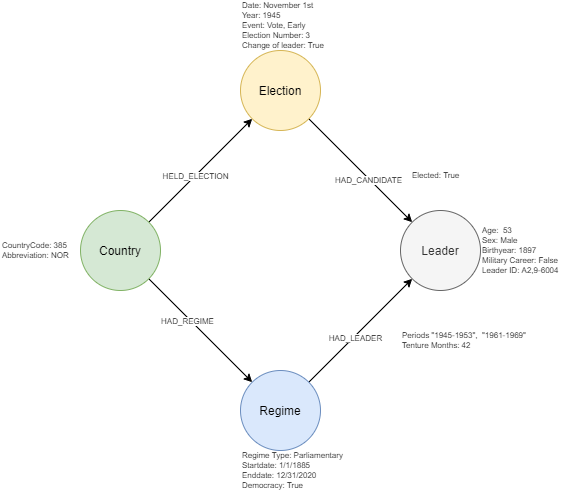
\includegraphics[scale=0.5]{images/milepael4/graph_database_base.drawio.png}
\end{figure}

\subsubsection{Hvorfor grafdatabase?}
Vi tenkte at grafdatabase er godt egnet for å se hvilke styringsmåter forskjellige land har. Det gir 
også en god oversikt over hvilke ledere som har styrt hvor, og eventuelt om de har styrt andre 
steder. Siden det ikke er for omfattende informasjon om hver node, kan de lett lagres som 
egenskaper. Det gjør det også lett å få oversikt på presteringen av hver leder og hvert land.

\subsubsection{Dataobjekter}
% Aggregering 1 %
\textbf{Regime Type By Popularity}\\
Denne framstiller populariteten blant de forskjellige Regjeringstypene ved å telle opp land.

\FigureCounter
\begin{figure}[H]
  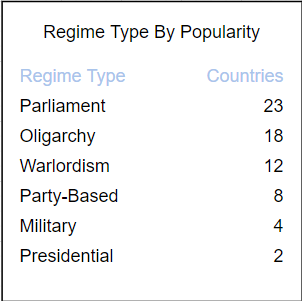
\includegraphics[scale=0.5]{images/milepael4/regimeTypeByPopularity.png}
\end{figure}

\textbf{Pseudo-Kode}
\begin{enumerate}
  \item Count countries relating to each regime type
  \item Group by tegime type
\end{enumerate}

% Aggregering 2 %
\textbf{Regime Type Development}\\
Denne komponenten viser utviklingen de forskjellige regjeringstypene gjennom årene. I 
framstillingen brukes et linjediagram.

\FigureCounter
\begin{figure}[H]
  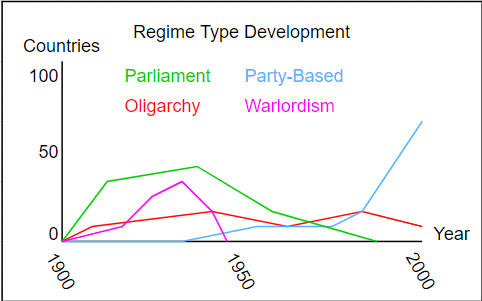
\includegraphics[scale=0.75]{images/milepael4/regimeTypeDevelopment.png}
\end{figure}

\textbf{Pseudo-Kode}
\begin{enumerate}
  \item Get regime types
  \item Count amount of countries relating to a regime type
  \item Group by year
\end{enumerate}

% Aggregering 3 %
\textbf{Most Influential Leader}\\
Most Influential Leader viser kun ett resultat. Dette er den lederen som totalt sett har vært oppnådd 
mest basert på antall Regimer og hvor lenge de har holdt på.

\FigureCounter
\begin{figure}[H]
  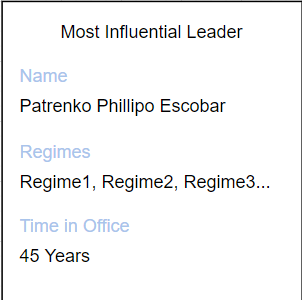
\includegraphics[scale=0.75]{images/milepael4/mostInfluentialLeader.png}
\end{figure}

% Aggregering 4 %
\textbf{Country By Regime Count w/ Regime}\\
Dette objektet fremstiller landene som har hatt flest regimer gjennom tidene, i tillegg til 
Regjeringstypene.

\FigureCounter
\begin{figure}[H]
  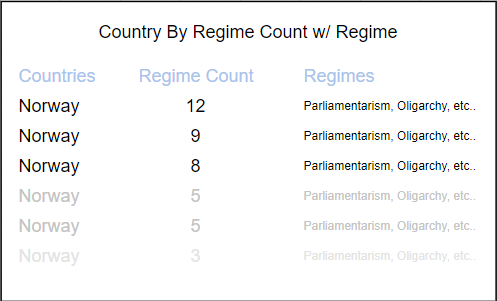
\includegraphics[scale=0.75]{images/milepael4/countryByRegimeCountWithRegime.png}
\end{figure}

\textbf{Pseudo-Kode}
\begin{enumerate}
  \item Get Countries and Regimes
  \item Sum Regime by Countries
  \item Group by countries
\end{enumerate}

\subsubsection{Operasjoner}



\subsubsection{Hvordan eksisterende data oppdateres}
I vår løsning for grafdatabaser lagres ikke komponentene direkte i databasen som objekter, men blir 
heller laget via queries. Derfor er det ikke samme behov for et rådata-objekt for å oppdatere disse 
komponenetene. Måten vi tenker at dette gjøres er at brukeren oppretter en ny node som skal 
plottes inn i databasen. For eksempel, kan brukeren opprette en ny leder-node med tilhørende 
properties, og det er denne som sendes til databasen.